\section{Introduction}
\label{sec:intro}

% Mobile wireless networks have witnessed substantial growth (1G to 6G), solidifying their position as one of the fastest-growing fields and playing a crucial role in advancing the information society. Wireless network systems can serve many devices accessing simultaneously, such as smartphones, IoT devices, autonomous vehicles, and intelligent infrastructure.
% %~\cite{8663985, 9779322}. 
% An example is a scenario in a smart city~\cite{HERATH2022100076}, where multiple smartphones, autonomous vehicles, surveillance cameras, and IoT devices form a dynamic network to exchange real-time data and coordinate their actions to optimize traffic flow and ensure public safety. Each client communicates wirelessly with each other and the central control system to achieve efficient and coordinated operations. Such network systems are critical in many application domains, from transportation and surveillance to industrial automation and environmental monitoring. As these systems grow in complexity and scale, managing the flow of data and optimizing network performance becomes increasingly challenging. 
% To this end, Multipath Transport Protocols (MTP) \nguyen{cite MPTCP and MPWUIC} have emerged as potential solutions enabling the use of multiple transmission paths at the same time, thereby maximizing the network utilization. 

% Le & Trung's text
%In the ever-evolving context of communication technologies, the transition to 5G and beyond has ushered in a new era of possibilities and challenges in wireless networks. Amidst this development, Multipath QUIC (MPQUIC)~\cite{mpquic,mpquic2} has emerged as a potential multipath transport protocol, changing to how mobile clients harness the capabilities of diverse wireless networks (e.g, Wi-Fi and cellular). By enabling seamless and simultaneous utilization of these networks, MPQUIC holds the promise of substantially elevating data transmission performance, bolstering connectivity, and improving the end-user experience.

%Kien's text 2023 Sep. 3
In the ever-evolving context of wireless communication technologies, the transition to 5G and beyond has ushered in a new era of possibilities and challenges. Amid this development, MPQUIC~\cite{mpquic,mpquic2} is emerging as a potential multipath transport protocol that changes how to harness the resources of available wireless networks on mobile clients (e.g., Wi-Fi and cellular). By enabling seamless and simultaneous utilization of these networks, MPQUIC promises to substantially elevate data transmission performance, bolster connectivity, and improve the clients' quality of experience. The default scheduler in MPQUIC is minRTT, which selects the path with the shortest round-trip time (RTT) and available congestion window (CWND) for packet transmission. However,  the minRTT-based scheduler's selection criteria possibly ignore better paths about to become available, especially in dynamic wireless networks. 

% Le & Trung's text
%One of the most crucial issues in handling MPQUIC is how to decide which path used at each time slot, i.e., path scheduling. 
%Conventionally, minRTT is adopted as the default scheduler in MPQUIC. 
%The minRTT-based scheduler chooses the path with the shortest round-trip time (RTT) and available CWND for packet transmission. 
%As a result, the minRTT-based scheduler always chooses the currently available path with the lowest RTT, possibly ignoring faster paths that are about to become available.

%However, this approach might not be optimal for heterogeneous wireless networks because the overall transmission time can be shortened by sending on a higher-RTT path, even if the lower-RTT path is available. 
%A novel multipath transport protocol is the Multipath QUIC (MPQUIC), recently introduced by~\cite{mpquic}, which presents an opportunity to enhance data transmission performance and reliability in wireless networks. 
% One of the critical aspects of MPQUIC is in how-to data distribution over multiple paths depending on the availability of network resources. Hence, it is essential to have an efficient scheduler that can optimize data transmission time, especially in an environment with varying conditions.
% MPQUIC scheduling algorithms fall under two categories: non-learning and learning-based approaches. Non-learning schedulers utilize packet-based events (such as one-way delay, packet loss rate, and available congestion window (CWND)) to determine the transmission strategy.
%A non-learning scheduler, minRTT, serves as the default in MPQUIC. 
%The minRTT scheduler selects the lower round trip time (RTT) path which is available CWND, to send packets. 
%However, this approach might not be optimal for heterogeneous wireless networks because the overall transmission time can be shortened by sending on a higher-RTT path, even if the lower-RTT path is available. 

%Le and Trung's text
%To address this issue, several schedulers, such as the Blocking Estimation-based MPTCP Scheduler (BLEST)~\cite{blest} and Earliest Completion First (ECF)~\cite{ecf}, are proposed. These schedulers introduce a waiting mechanism to evaluate whether sending on the higher-RTT path or waiting for the lower-RTT path would yield better results.
%However, the primary drawback of the aforementioned schedulers is their inability to handle networks with high levels of network dynamicity, i.e., significant variation in latency or packet loss~\cite{wifilte}. 
%Indeed, as these schedulers rely on predetermined scheduling strategies, they cannot adapt to the change of network conditions. 
%% in networks with high dynamicity levels, i.e., significant variation in latency or packet loss, these schedulers may only partially exploit the benefits of multipath transport and result in not optimal performance~\cite{peekaboo}. 
%To this end, learning-based schedulers~\cite{peekaboo, 10.1145/3568562.3568654} have been introduced recently.Most learning-based schedulers employ reinforcement learning models to select transmission paths. In~\cite{peekaboo}, the authors introduce Peekaboo, which exploits multi armed bandit algorithm to determine the transmisison path when the lowest-RTT path is not available. The authors in~\cite{10.1145/3568562.3568654} implement q-ReLeS, which is a deep reinforcement learning-based scheduler for MPQUIC. q-ReLeS leverages historical and current network states to determine transmission path.
%%\nguyen{describe about other learning-based schedulers here. For each, write 2-3 sentences about its main idea.}

%Kien's text 2023 Sep. 3
There are efforts to develop MPQUIC schedulers to adapt better in wireless networks, which are roughly classified as non-learning and learning categories. The former includes the Blocking Estimation-based MPTCP Scheduler (BLEST)~\cite{blest} and Earliest Completion First (ECF)~\cite{ecf}, etc., which introduce a waiting mechanism to evaluate whether sending on the higher-RTT path or waiting for the lower-RTT one would yield better results. The primary drawback of the schedulers above is their inability to handle networks with high levels of network dynamicity, i.e., significant variation in latency or packet loss~\cite{wifilte}. That is because they rely on predetermined scheduling strategies that cannot correctly adapt to the change in network conditions. To better cope with such situations, the approach in the latter category has been introduced recently~\cite{peekaboo, 10.1145/3568562.3568654}. The learning-based schedulers employ reinforcement learning models to select transmission paths. In~\cite{peekaboo}, the Peekaboo scheduler exploits a multi-armed bandit algorithm to determine the transmission path when the lowest-RTT path is unavailable. In~\cite{10.1145/3568562.3568654}, the authors introduced q-ReLeS, a deep reinforcement learning-based scheduler, which leverages historical and current network states for path scheduling.

% Le & Trung's text
%Although learning-based algorithms can adapt to network changes quite well, they, like non-learning schedulers, suffer from a critical drawback: they all only consider network scenarios with a single client. In practice, however, clients often share the same network resources concurrently. Multiple clients may retrieve data simultaneously from a server, for instance. In such a context, using uni-client-oriented schedulers will likely cause a problem that we call selfish scheduling, as depicted in~\figref{fig:multiclient}. Specifically, all client schedulers will attempt to select the optimal path, causing congestion on that path while leaving other paths unused. Motivated by this observation, in this work, we are the first to investigate the scheduling problem for the MPQUIC protocol in the presence of multiple clients. We then leverage the reinforcement learning paradigm and propose a Q-learning-based scheduler capable of simultaneously scheduling the packets of multiple clients. When determining the transmission path for each packet, our scheduler considers all clients' presence to optimize download time and loss rate for all client flows. 

% Kien's text 2023 Sep. 3
Although the previous learning-based MPQUIC schedulers improve MPQUIC performance in dynamic networks, they (including non-learning ones) usually simplify or consider a simple network model with only one client. In practice, however, several MPQUIC clients may retrieve data simultaneously from a server on shared networks. In such a context, using the existing schedulers will likely cause a problem that we call rush scheduling, as depicted in~\figref{fig:multiclient}.
Specifically, all instance schedulers will attempt to select the optimal path (for one client), causing congestion on that path while leaving others unused. Motivated by this observation, this work investigates the MPQUIC scheduling problem in the presence of multiple clients. We then leverage the reinforcement learning paradigm in designing an MPQUIC scheduler capable of simultaneously scheduling multiple clients' upcoming transmissions. The scheduler considers all clients' presence to optimize download time and loss rate for all client flows. 
\begin{figure}[t]
\centering
 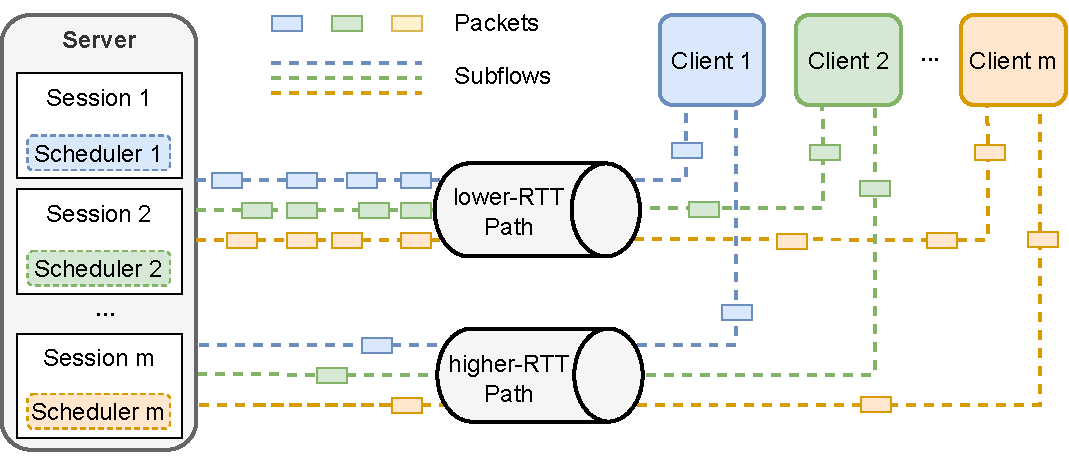
\includegraphics[width=8.8cm]{figs/ccnc-intro.pdf}
\caption{\textbf{An illustration of the rush scheduling phenomenon.} As all schedulers strive for the best path (i.e., lower-RTT Path), this path is congested while the other (i.e., higher-RTT Path) remains unused. } \label{fig:multiclient}
%\vspace{-0.1cm}
\end{figure}
The contributions of our work are as follows.
\begin{itemize}
    \item We are the first to identify the rush scheduling phenomenon and study the multi-client scenario in path scheduling problems for multipath transport protocols. 
    \item We propose MuLeS, a Q-learning-based multi-client scheduler for MPQUIC. MuLeS makes decisions based on observations of the overall state of the network via a central controller. By leveraging the self-learning ability of reinforcement learning, MuLeS can gradually learn and dynamically adjust its scheduling decisions based on real-time network conditions and performance metrics. Moreover, by considering the states of all flows, MuLeS can offer globally optimal decisions for all clients.
 % Le & Trung's text   
  %  \item We perform extensive experiments using simulation to evaluate the efficacy of MuLeS and compare it to that of other schedulers. The results demonstrate that our proposal is superior to existing methods regarding multiple metrics, including download time and loss rate.
%Kien's text
   \item We extensively evaluate the efficacy of MuLeS by using simulation in comparison to other schedulers. The results demonstrate that MuLes is superior to existing methods regarding download time and loss rate.
\end{itemize}
The remainder of this paper is as follows. \sectionref{sec:background} provides background and the related works. We describe the design of MuLeS, evaluation in \sectionref{sec:proposal},  \sectionref{sec:evaluation}, respectively. Finally, \sectionref{sec:conclusion} concludes the paper. 


